\documentclass[10pt,twocolumn]{article}
\usepackage[margin=0.58in]{geometry}
\usepackage{graphicx}
\usepackage{booktabs}
\usepackage{amsmath}
\usepackage{microtype}
\usepackage{xcolor}
\usepackage{enumitem}

\setlength{\parskip}{2pt}
\setlength{\parindent}{9pt}
\setlist[itemize]{leftmargin=*,topsep=1pt,itemsep=0pt}
\pagenumbering{gobble}

\newcommand{\engram}{\textsc{Engram}}
\newcommand{\bfactor}{\mathrm{BF}}

\title{\vspace{-0.55in}\textbf{A Sparse N-Gram Memory Path for Small GPT Training}}
\author{rom\_rwom internal report}
\date{June 16, 2026}

\begin{document}
\maketitle
\vspace{-0.18in}

\begin{abstract}
We summarize the current \engram{} memory path in the modded-nanogpt
experiments.  The best historical 1500-step validation loss observed in this
line is \textbf{3.2411} with a BF400 trigram-heavy table, hit-scaled reads, and
memory-head normalization.  The later extracted SOTA-control stack, used for
the cleaned implementation path, reaches \textbf{3.2440} on its best seed and
has a seven-seed spread of 3.2440--3.2478.  The central result is structural:
large sparse n-gram tables help, but only when row allocation, layer addressing,
normalization, and optimizer state are shaped to avoid hot-row collapse and
late over-coupling.
\end{abstract}

\section{Architecture}
The model keeps the dense GPT mostly intact and adds a learned sparse memory
readout at selected residual layers.  For the current extracted SOTA path, the
memory is read at layers 2 and 8.  Each token position forms bigram and trigram
hashes, each hash addresses a row in a large learned table, and the retrieved
rows are projected into per-head key/value vectors.  A normalized hidden state
queries the retrieved key; the resulting scalar gate modulates the value before
the heads are mixed and added through the residual path.

\begin{figure}[t]
\centering
\fbox{\begin{minipage}{0.94\linewidth}
\small
\begin{center}
\textbf{SOTA \engram{} readout path}
\end{center}
\vspace{-0.05in}
\[
\begin{array}{c}
\text{tokens } x_{1:t},\; h_t \\
\Downarrow \\
\text{bigram/trigram hashes, layer-specific salts} \\
\Downarrow \\
\text{K=2 row superposition: base row } + 0.5\,\text{aux row} \\
\Downarrow \\
\text{normalize memory heads; per-head } K,V \text{ projections} \\
\Downarrow \\
g=\sqrt{|q^\top k|}\,\mathrm{sign}(q^\top k),\quad
\mathrm{out}=\sum_h \sigma(g_h)V_h \\
\Downarrow \\
\text{head mix }(0.5,-0.5),\ \text{short conv},\ \text{normalized readout}
\end{array}
\]
\vspace{-0.08in}
\end{minipage}}
\caption{The cleaned extraction covers this branch exactly: K=2 superposed
n-gram rows, no row signs, layer-specific hashes and readout deltas, scalar
Adam-compatible sparse rows, and normalized memory/readout.}
\end{figure}

The strongest historical BF400 configuration used:
{\small
\begin{itemize}
\item \texttt{ROM\_LAYERS=2,8}, \texttt{ENGRAM\_DIM=768}, one memory head.
\item Bigram/trigram row factors $(0.5,1.5)$, giving more rows to trigrams.
\item Layer-specific hashes/readouts with shared row address capacity
(\texttt{ENGRAM\_LAYER\_PARTITION\_GROUPS=1}).
\item Hit-scaled readout with exponent 0.25 and mean normalization.
\item Memory-head and output-readout RMS normalization.
\item Sparse scalar Adam for memory rows, enabling BF400 within a 96 GB GPU.
\end{itemize}}

\section{SOTA Trace}
Table~\ref{tab:sota} separates the best historical result from the later
current-code SOTA-control stack.  This matters because the project accumulated
small implementation changes while we were cleaning and extracting the code.
Single-seed deltas below a few thousandths are therefore treated as noise unless
they replicate across matched seeds.

\begin{table}[t]
\centering
\small
\resizebox{\linewidth}{!}{%
\begin{tabular}{lccc}
\toprule
Run family & BF & seeds & val loss \\
\midrule
Historical best, trigram-heavy + hit read & 400 & 5 & \textbf{3.2411} \\
Checkpoint replay of same line & 400 & 5 & 3.2413 \\
Current-code SOTA control, best seed & 300 & 5 & \textbf{3.2440} \\
Current-code SOTA controls, seed mean & 300 & 5--11 & 3.2453 \\
Current-code SOTA controls, range & 300 & 5--11 & 3.2440--3.2478 \\
\bottomrule
\end{tabular}
}
\caption{1500-step validation-loss anchors.  The current-code seed sweep
estimates the noise floor for later structural comparisons.}
\label{tab:sota}
\end{table}

\section{BF Sweep}
The BF sweep asks whether simply widening the sparse table keeps paying off.
It does, but with diminishing returns and substantial memory cost.  The
current-meta sweep moved from 3.2596 at BF40 to 3.2462 at BF400, while table
parameters grew from 1.55B to 15.45B and peak memory from 29.8 GiB to 89.8 GiB.

\begin{figure}[t]
\centering
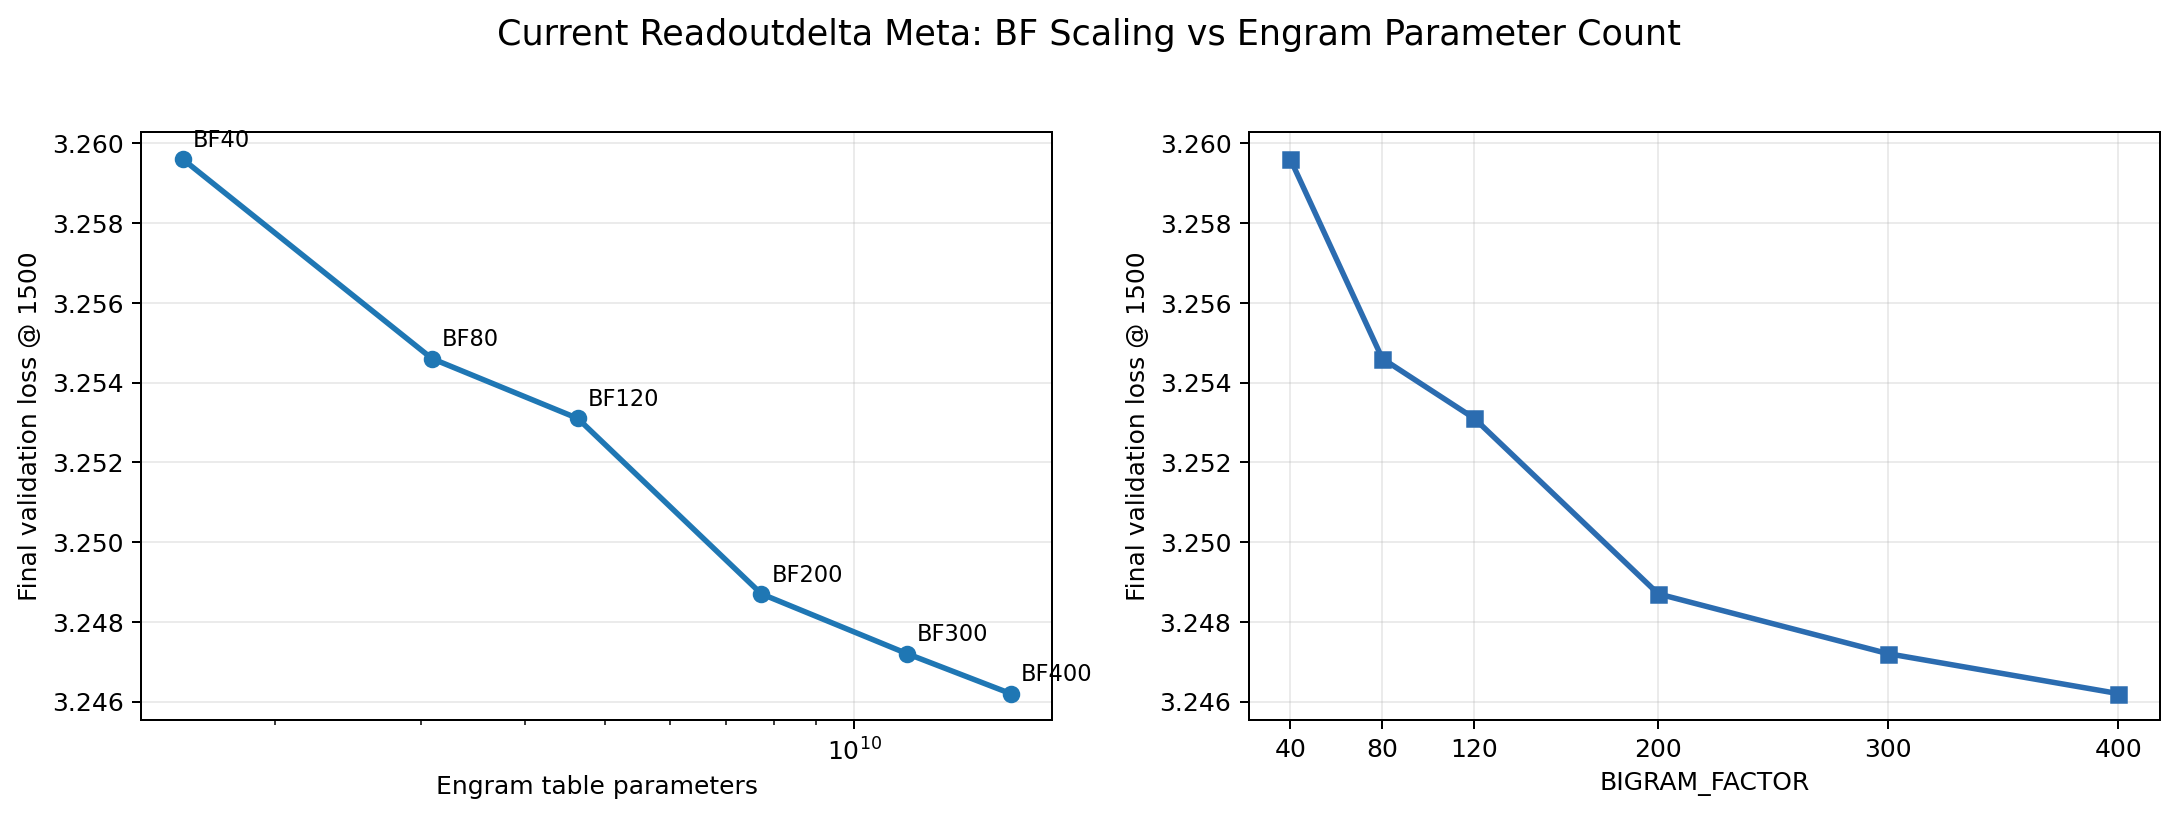
\includegraphics[width=\linewidth]{../bf_sota_scaling_20260609/bf_current_meta_bfscale_vs_params.png}
\caption{Current-meta BF sweep: validation improves as table row count grows,
but gains flatten past BF200--BF300.  This motivated structural changes rather
than only larger tables.}
\label{fig:bfsweep}
\end{figure}

\begin{table}[t]
\centering
\small
\begin{tabular}{rrrrr}
\toprule
BF & val & table params & peak GiB & touched \\
\midrule
40  & 3.2596 & 1.55B  & 29.1 & 22.2\% \\
80  & 3.2546 & 3.09B  & 34.9 & 11.9\% \\
120 & 3.2531 & 4.64B  & 40.7 & 8.1\% \\
200 & 3.2487 & 7.73B  & 52.3 & 4.9\% \\
300 & 3.2472 & 11.59B & 66.8 & 3.3\% \\
400 & 3.2462 & 15.45B & 87.7 & 2.5\% \\
\bottomrule
\end{tabular}
\caption{BF scaling summary for the current-meta stack.  ``Touched'' is the
fraction of rows hit during the run.}
\end{table}

\section{What Moved}
Three interventions carried most of the progress.  First, scalar-row Adam made
large tables affordable; vector moments were memory-expensive, while row-scalar
moments preserved enough adaptivity to train BF400.  Second, sharing the row
address space across L2/L8 while keeping layer-specific hashes/readouts was a
robust structural win: it improved the earlier four-seed mean from about 3.2463
to about 3.2447.  Third, memory-head normalization and trigram-heavy allocation
matched the observed structure of the table: outputs are dominated by a small
set of frequently touched rows, and trigrams benefit from more capacity.

Several plausible ideas did not become reliable SOTA movers.  Extra memory
layers improved some early checkpoints but failed or tied by final loss.
Count-sketch and combine-mix variants produced interesting distributed-code
behavior, but final losses remained inside the current SOTA-control seed band.
Row pruning showed that many cold rows can be recovered as space, but did not by
itself explain or improve the loss frontier.

\section{Extraction Status}
The SOTA memory branch has now been extracted into a slim implementation.  A
local equivalence harness instantiates the legacy \texttt{train\_gpt.py}
\engram{} class and the new extracted module at small dimensions, copies the
same state dict, and checks random readouts for layers 2 and 8.  The extracted
branch matches the legacy path exactly on tested token lengths, with maximum
absolute difference 0.0.  This gives a stable base for moving the remaining GPT
wrapper out of the monolithic training file without losing the verified SOTA
readout semantics.

\end{document}
